%%
%% This is file `sample-acmsmall-conf.tex',
%% generated with the docstrip utility.
%%
%% The original source files were:
%%
%% samples.dtx  (with options: `acmsmall-conf')
%% 
%% IMPORTANT NOTICE:
%% 
%% For the copyright see the source file.
%% 
%% Any modified versions of this file must be renamed
%% with new filenames distinct from sample-acmsmall-conf.tex.
%% 
%% For distribution of the original source see the terms
%% for copying and modification in the file samples.dtx.
%% 
%% This generated file may be distributed as long as the
%% original source files, as listed above, are part of the
%% same distribution. (The sources need not necessarily be
%% in the same archive or directory.)
%%
%%
%% Commands for TeXCount
%TC:macro \cite [option:text,text]
%TC:macro \citep [option:text,text]
%TC:macro \citet [option:text,text]
%TC:envir table 0 1
%TC:envir table* 0 1
%TC:envir tabular [ignore] word
%TC:envir displaymath 0 word
%TC:envir math 0 word
%TC:envir comment 0 0
%%
%%
%% The first command in your LaTeX source must be the \documentclass
%% command.
%%
%% For submission and review of your manuscript please change the
%% command to \documentclass[manuscript, screen, review]{acmart}.
%%
%% When submitting camera ready or to TAPS, please change the command
%% to \documentclass[sigconf]{acmart} or whichever template is required
%% for your publication.
%%
%%
\documentclass[acmsmall]{acmart}

%%
%% \BibTeX command to typeset BibTeX logo in the docs
\AtBeginDocument{%
  \providecommand\BibTeX{{%
    Bib\TeX}}}

%% Rights management information.  This information is sent to you
%% when you complete the rights form.  These commands have SAMPLE
%% values in them; it is your responsibility as an author to replace
%% the commands and values with those provided to you when you
%% complete the rights form.
%\setcopyright{acmcopyright}
%\copyrightyear{2018}
%\acmYear{2018}
%\acmDOI{XXXXXXX.XXXXXXX}

%% These commands are for a PROCEEDINGS abstract or paper.
\acmConference[Robotics'23, Master CS]{}{Spring 2023}{Leiden, the Netherlands}
%%
%%  Uncomment \acmBooktitle if the title of the proceedings is different
%%  from ``Proceedings of ...''!
%%
%%\acmBooktitle{Woodstock '18: ACM Symposium on Neural Gaze Detection,
%%  June 03--05, 2018, Woodstock, NY}

%%
%% For managing citations, it is recommended to use bibliography
%% files in BibTeX format.
%%
%% You can then either use BibTeX with the ACM-Reference-Format style,
%% or BibLaTeX with the acmnumeric or acmauthoryear sytles, that include
%% support for advanced citation of software artefact from the
%% biblatex-software package, also separately available on CTAN.
%%
%% Look at the sample-*-biblatex.tex files for templates showcasing
%% the biblatex styles.
%%

%%
%% The majority of ACM publications use numbered citations and
%% references.  The command \citestyle{authoryear} switches to the
%% "author year" style.
%%
%% If you are preparing content for an event
%% sponsored by ACM SIGGRAPH, you must use the "author year" style of
%% citations and references.
%% Uncommenting
%% the next command will enable that style.
%%\citestyle{acmauthoryear}

\usepackage{subcaption}

%%
%% end of the preamble, start of the body of the document source.
\begin{document}

%%
%% The "title" command has an optional parameter,
%% allowing the author to define a "short title" to be used in page headers.
\title[Autonomous Driving Copilot]{Autonomous driving copilot: Gesture control and autonomous driving system}

%%
%% The "author" command and its associated commands are used to define
%% the authors and their affiliations.
%% Of note is the shared affiliation of the first two authors, and the
%% "authornote" and "authornotemark" commands
%% used to denote shared contribution to the research.
\author{Siwen Tu}
\author{Lin He}
\author{Ruilin Ma}
\author{Chenyu Shi}
\author{Shupei Li}

\affiliation{%
  \institution{Team: $<$ Pi team $>$}
  \country{LIACS}
}

%%
%% By default, the full list of authors will be used in the page
%% headers. Often, this list is too long, and will overlap
%% other information printed in the page headers. This command allows
%% the author to define a more concise list
%% of authors' names for this purpose.
\renewcommand{\shortauthors}{S. Tu, L. He, R. Ma, C. Shi and S. Li}

%%
%% The abstract is a short summary of the work to be presented in the
%% article.
\begin{abstract}
    \textbf{Abstract}. Traffic accidents are a severe problem all over the world. Given this situation, we design an autonomous driving copilot consisting of gesture control and autonomous driving system. In this paper, we explain the methodology we apply to these two systems and show the demo process. At the end of the paper, we discuss the achievements of our project and proposed possible improvements in future work.
\end{abstract}

%%
%% The code below is generated by the tool at http://dl.acm.org/ccs.cfm.
%% Please copy and paste the code instead of the example below.
%%

%%
%% Keywords. The author(s) should pick words that accurately describe
%% the work being presented. Separate the keywords with commas.
\keywords{Autonomous driving; Gesture control; Raspberry car; Opencv}

%%
%% This command processes the author and affiliation and title
%% information and builds the first part of the formatted document.
\maketitle

\section{Introduction}
Approximately 1.3 million people die each year in traffic accidents~\cite{who-road-traffic-injuries}. Autonomous driving holds great potential to mitigate this issue by automatically detecting obstacles, planning routes intelligently, and driving with greater discipline. In order to assist real-world driving, we have developed a gesture control system that simulates the driving process, allowing drivers to learn and become familiar with various driving scenarios. Additionally, to address the common challenge of parking difficulties, we have designed an autonomous parking system. This system aims to provide a solution for individuals who struggle with parking their cars.

This paper is divided into two main parts: gesture control and autonomous parking. In the gesture control section, we provide a detailed explanation of the mechanism used to recognize gestures captured by the computer camera. We discuss the process of generating and transmitting commands, as well as executing these commands on the car. In the autonomous parking section, we outline the methodology employed for object detection and route planning. To showcase the outcomes of our project, we include demo screenshots that effectively demonstrate the results achieved. We also record a short video demo of our project, which can be downloaded from \url{https://drive.google.com/file/d/1P_EU3GSJ-22wRUMosOGIXMXBX2ZPh0tL/view?usp=sharing}. The source code and documents of our project can be accessed on GitHub: \url{https://github.com/ShupeiLi/robotics}.

\section{Gesture control}
During the gesture control stage, the driver sits in front of the computer, observes the road condition through the video stream sent from the raspberry pi mobile car, and controls the movement of the car via gestures. The key part of gesture control is correctly identifying gestures in a short time. Our solution is using the CVZone package's implementation of the MediaPipe Hands model \cite{cvzone}.

The MediaPipe Hands model is a pipeline designed for detecting landmarks of hands in images or videos. It is composed of two stages. The first stage is marking a square area where palms are present with a single-shot palm detector. And the second stage is recognizing the handedness and the landmarks of hands with an encoder-decoder-based tracker. Note that the handedness is a flag indicating whether the detected hand is left or right. The landmarks of hands provide critical information for restoring gestures. The MediaPipe Hands model adopts the topology suggested by \cite{hand} and returns the 21 landmarks, which are shown in Figure \ref{fig:hand}. The basic building block of the detector and the tracker is the convolutional neural network. The MediaPipe Hands model has been pre-trained on three large gesture datasets and added as a module in the MediaPipe framework.

\begin{figure}[!ht]
    \centering
    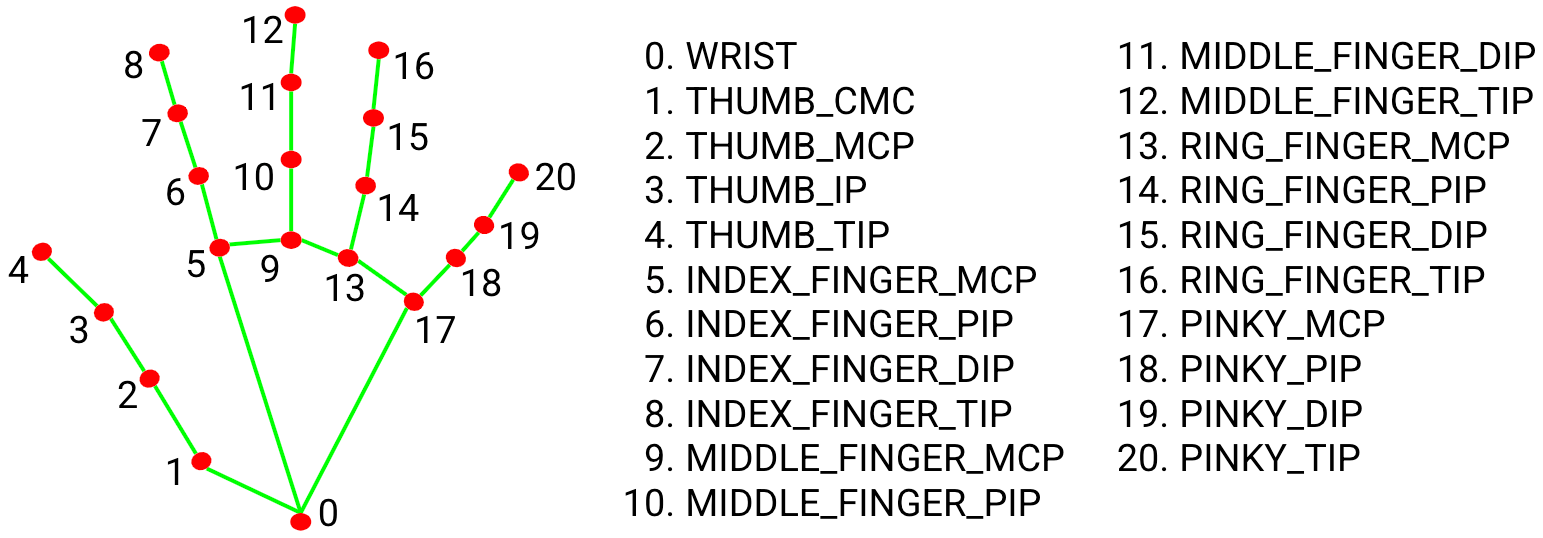
\includegraphics[width=11cm]{./hand.png}
    \caption{The topology of the hand \cite{google}.}
    \label{fig:hand}
\end{figure}

The control logic of our algorithm mainly utilizes the number and the relative height of hands. CVZone provides APIs that can return a list of detected hands and extract the center coordinates of hands from 21 landmarks. The gesture control program will only be activated if two hands are appearing in front of the computer camera, which simulates the scenario of driving a real car by steering the wheel. When the number of hands is less than two, which indicates that the driver is not ready to start or wishes to stop, the program will brake the mobile car immediately. Our program supports three motion commands: turn left, turn right, and go straight. We use the relative height of two hands to determine the intent of the driver. Denote the $y$ coordinate of the center of the left hand as $y_{\text{left}}$ and that of the right hand as $y_{\text{right}}$. Given a threshold $\eta$, we regard the driver wants to turn left if $y_{\text{right}} > y_{\text{left}} + \eta$ or turn right if $y_{\text{left}} > y_{\text{right}} + \eta$. In other cases, we regard the driver wants to go straight. We set the $\eta$ to 200 according to testing results. If the driver wants to stop or switch to the autonomous driving mode, he or she just needs to move hands outside the view of the camera to deactivate the gesture control program. Figure \ref{fig:gesture-control} illustrates the effect of the gesture control program in action. Monitor screens of the computer camera and the car's camera are shown on the left side of the screenshot. The right side of the screenshot is the car going straight.
\begin{figure}[!ht]
    \centering
    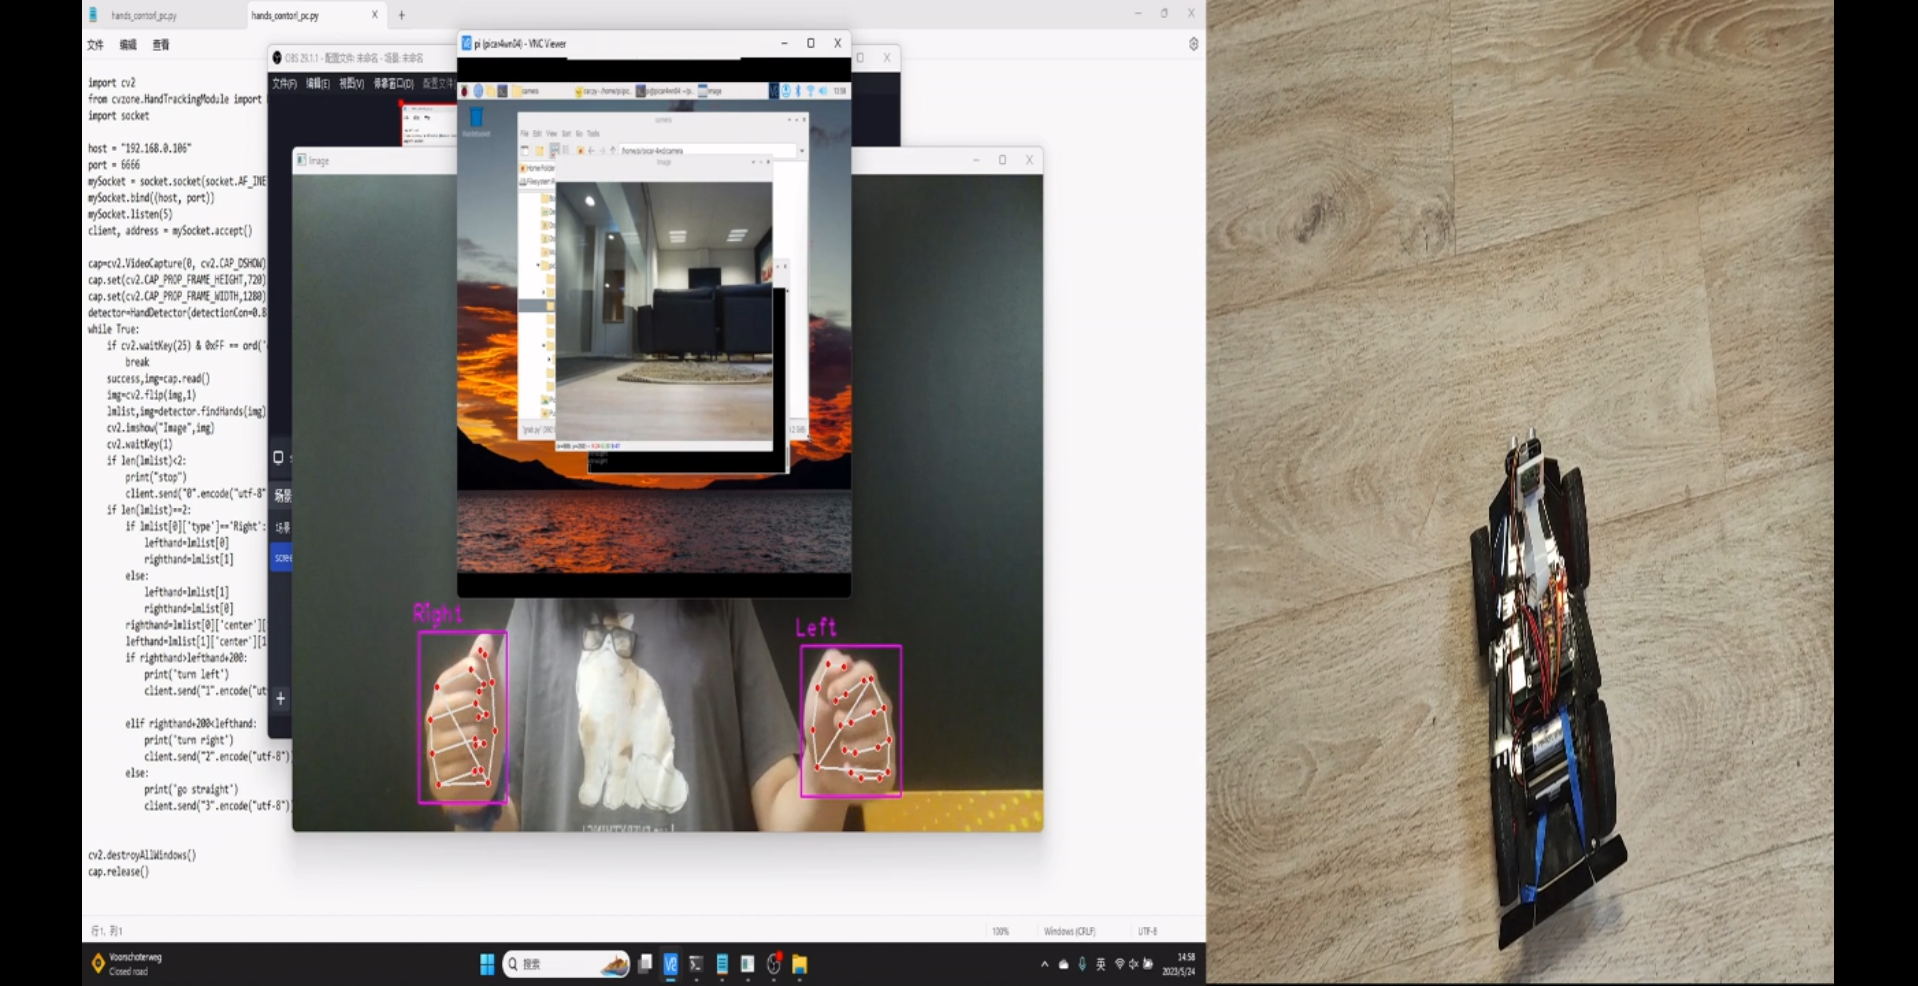
\includegraphics[width=13cm]{./gesture-control.png}
    \caption{Gesture control in action.}
    \label{fig:gesture-control}
\end{figure}

\section{Autonomous driving}
As showcased in the proposal, we aim at developing an autonomous driving system for the robot car to take actions without manual intervention in certain situations where manual control is proven to be difficult. We focus on one particular situation, namely reverse parking. In this particular task, the car needs generally four steps to achieve successful parking, which are marking line detection, positional adjustments and reserve parking, and stopping.

The marking detection process requires the robot car to detect the parking marking line. To achieve this, a color-based line-detection method is implemented. We took advantage of computer vision's powerful capabilities, particularly the HSV (Hue, Saturation, Value) color space. With its improved ability to represent colors intuitively in comparison to the traditional RGB color model, the HSV color model emerged as the ideal option for distinguishing objects under various lighting circumstances. We developed a reliable and effective object detection method that can quickly and effectively identify things of interest in real-time by utilizing the HSV color space. In HSV, Hue represents the color portion.\cite{HSV} The common color ranges can be represented as: Red $[0^\circ,60^\circ]$, Yellow $[61^\circ,120^\circ]$, Green $[121^\circ,180^\circ]$, Cyan $[181^\circ,240^\circ]$, Blue $[241^\circ,300^\circ]$, Magenta $[301^\circ,360^\circ]$. In our implementation, the following color is set for selection, namely \texttt{red, red\_2(light), orange, yellow, green, blue, purple}. 

Line detection is achieved with \texttt{OpenCV} and \texttt{Picamera} libraries, and is directly computed on board to increase its real-time performance. In each execution, one and only one color is selected, which corresponds to the real color of the marking line. Our test shows that the color of \texttt{orange} is the best working configuration, possibly due to its vibrant nature as it has the best sensitivity and robustness and therefore is set as the default color for detection. Once selected, the program will enable the car to perform 360-degree turns at the spot until the parking line with the selected color is spotted. In order to enable the vehicle to position relatively straight to the parking lot, we set a pixel threshold which counts the number of pixels of the colored line that is within the camera view. The idea is that we can use the actual length of the marking line (which in this case is represented by some colored tapes clung to the ground) to determine whether the vehicle is positioned rather perpendicular to the marking line. This will make the later process more accurate and easier to fulfill.

After the line is detected, the car will enter the positional adjustments and reserve parking phase. The car first stops for 2 seconds, reminding the driver of the fact that the line is detected. Then the car turns $180^\circ$ and ends up with the position that is completely reversed to the position as the line is detected so that the car can move reversely into the parking area. Following, the car stops for another 1 second before the car actually moves back. During the backward process, the line detection is always open. Same to the methodology utilized previously, the car will go back until the camera detected the line again, which is carried out in the stopping phase. The cease of backward requires firstly the line is detected meanwhile the pixel width of the line lies above 300 in the camera view. This is used as a positional reference to ensure that the car is fully in the parking region. At this point, autonomous driving will stop as the line width reaches the parking requirement. All phases are executed autonomously and do not require human intervention. Figure \ref{fig:ato} illustrates a screenshot of reverse parking in action. It can be seen that the marking line is detected at this moment and the car is preparing for its positional adjustments for a smooth reverse parking.

\begin{figure}[!ht]
    \centering
    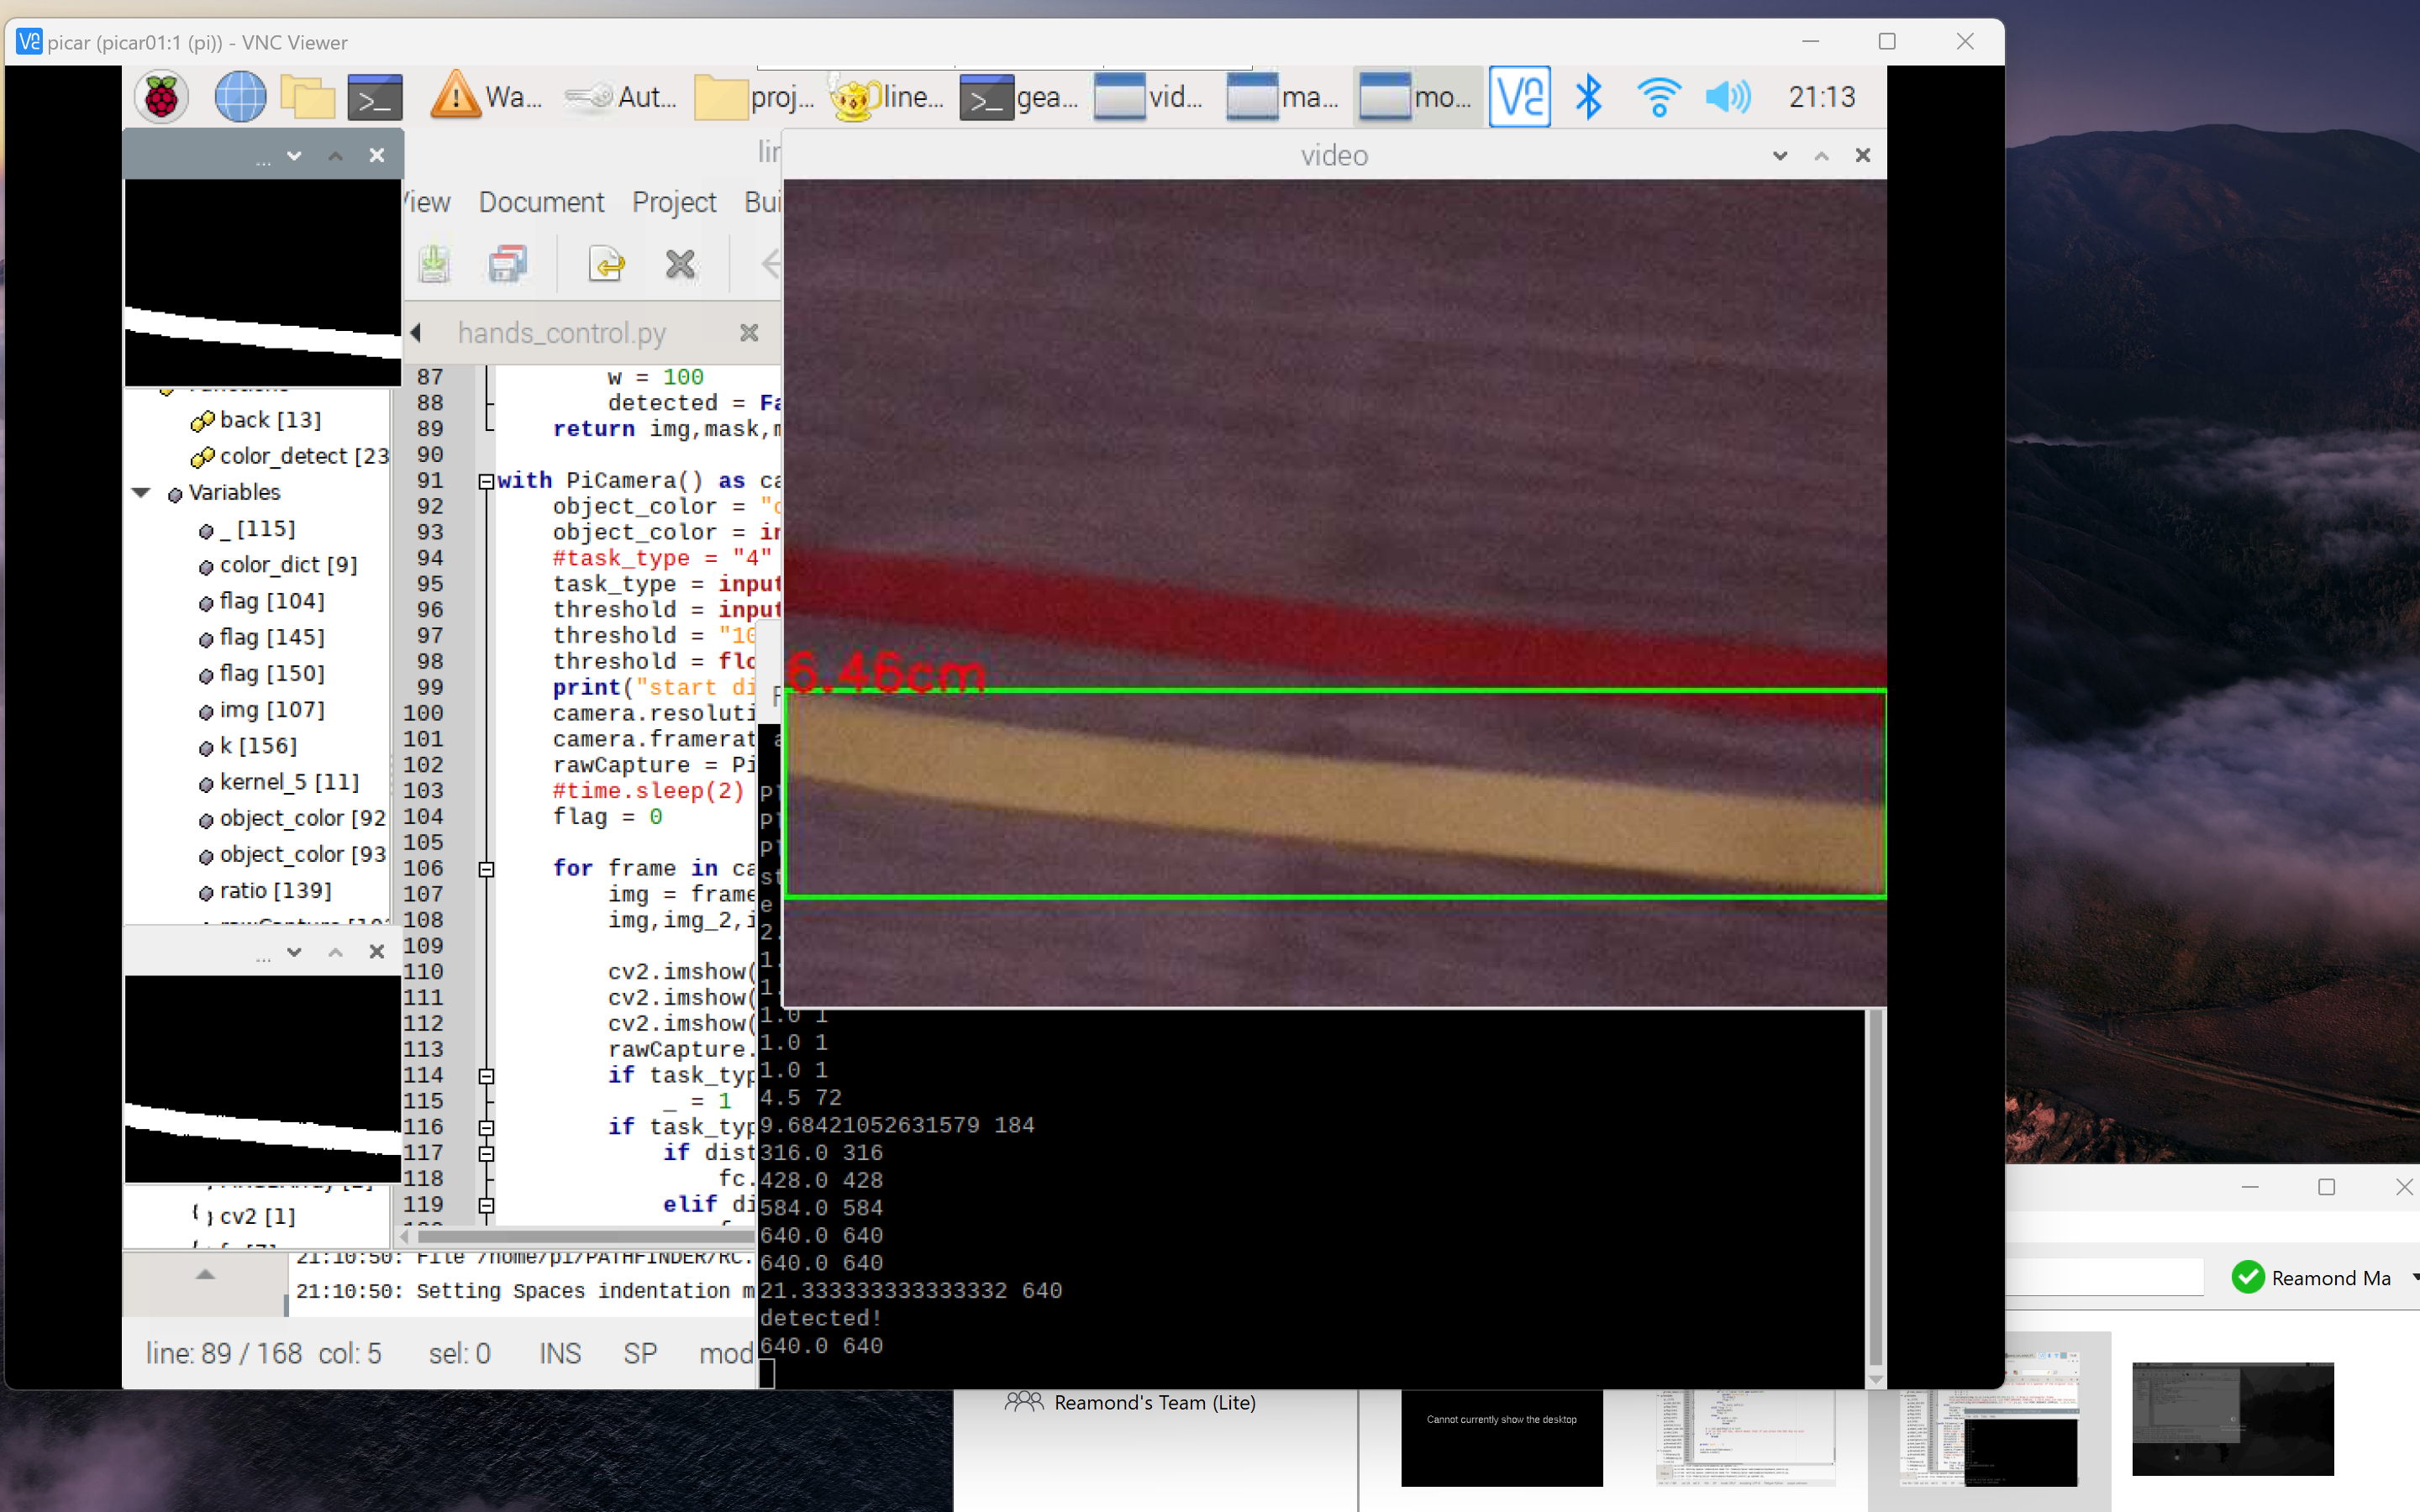
\includegraphics[width=13cm]{./action.png}
    \caption{Autonomous reserve parking in action. It can be noted that the marking line is detected and the vehicle is now preparing for positional adjustments.}
    \label{fig:ato}
\end{figure}

\section{Conclusion}

In this paper, we develop an autonomous driving copilot consisting of gesture control and autonomous driving to assist drivers in virtual and reality. As for gesture control, we utilize the CVZone package to implement gesture recognization, and the number and the relative height of hands to implement the control logic. As for autonomous driving, we utilize OpenCV and Picamera libraries to implement line detection and plan the routes for position adjustments and reverse parking. 

However, there are still potential areas for improvement in future work. For instance, in the gesture control interface, we could further develop additional functions to enable more precise control, such as reverse driving and a wider range of speed choices. Additionally, in the context of autonomous driving, the stability and robustness of line detection could be enhanced by implementing noise reduction techniques or transitioning to neural networks for more accurate detection.
%%
%% The next two lines define the bibliography style to be used, and
%% the bibliography file.
\bibliographystyle{ACM-Reference-Format}
\bibliography{main}

%%
%% If your work has an appendix, this is the place to put it.
\end{document}
\endinput
%%
%% End of file `sample-acmsmall-conf.tex'.
